\documentclass[letter]{article}
\usepackage[utf8]{inputenc}
\usepackage[spanish]{babel}

\usepackage{tikz}
\usetikzlibrary{shapes.geometric, arrows}
\graphicspath{ {images/} }
\usepackage{wrapfig}

%%importante ponerlo para tener español

\title{Practica 2}
\author{
Rubalcava Cortés Javier Roberto
\and 
Muñoz Carpio Erick David
}
\date{\today}

\usepackage{natbib}
\usepackage{graphicx}

\tikzstyle{startstop} = [rectangle, rounded corners, minimum width=3cm, minimum height=1cm,text centered, draw=black, fill=red!30]

%%\tikzstyle{io} = [trapezium, trapezium left angle=70, trapezium right angle=110, minimum width=3cm, minimum height=1cm, text centered, draw=black, fill=blue!30]
%%la comento por que de momento no la estamos usando
\tikzstyle{process} = [rectangle, minimum width=3cm, minimum height=1cm, text centered, draw=black, fill=orange!30]

\tikzstyle{arrow} = [thick,->,>=stealth]
\begin{document}

\maketitle
\begin{center}
    \textbf{Grupo:602}
\end{center}

\newpage

 
\tableofcontents{}
\newpage



\section{Objetivos.}

\begin{itemize}
    \item Efectuaras alguna recciones quimicas.
    \item Escribirás las ecuaciones completas de las reacciones que efectuaras y las
\end{itemize}

\section{Investigación previa.}
    \subsection{Nitrato cúprico.}
        \begin{wrapfigure}{l}{0.25\textwidth}
            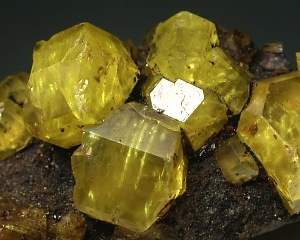
\includegraphics[width=1\linewidth]{azufre} 
            \caption{Axufre en forma de cristal}
            \label{fig:subim1}
        \end{wrapfigure}
        El azufre es el elemento numero 16 de la tabla periodica, ubicado en la X familia y en el Y grupo. Tiene una masa atomica de 32.065, ademas de tener propiedades electricas de aislante y una resistencia de Z.\par
        Se encuentra naturalmente en volcanes, cerca de aguas termales y meteoritos \par
        Algunos de los usos que tiene el Azufre es como fertilizante \cite{acuna1991fertilizacion}
        Lorem ipsum dolor sit amet, consectetur adipiscing elit. Duis id sem libero. Proin vitae purus rutrum, scelerisque turpis non, aliquam massa. Pellentesque vel cursus diam. Curabitur quis ligula nec enim sodales hendrerit. Donec sed risus ipsum. Aenean molestie aliquam nisi, eu eleifend velit bibendum non. Aenean venenatis ligula facilisis, pellentesque metus a, placerat orci. Morbi nec nibh eget turpis viverra mattis quis vel leo. Nunc et ligula sollicitudin, consectetur arcu sed, cursus nisl. Fusce congue porta lorem quis fermentum. Fusce congue eu justo sit amet facilisis.\par
    \subsection{Óxido cúprico.}
        Lorem ipsum dolor sit amet, consectetur adipiscing elit. Duis id sem libero. Proin vitae purus rutrum, scelerisque turpis non, aliquam massa. Pellentesque vel cursus diam. Curabitur quis ligula nec enim sodales hendrerit. Donec sed risus ipsum. Aenean molestie aliquam nisi, eu eleifend velit bibendum non. Aenean venenatis ligula facilisis, pellentesque metus a, placerat orci. Morbi nec nibh eget turpis viverra mattis quis vel leo. Nunc et ligula sollicitudin, consectetur arcu sed, cursus nisl. Fusce congue porta lorem quis fermentum. Fusce congue eu justo sit amet facilisis.\par
    \subsection{Hidróxido cúprico.}
        Lorem ipsum dolor sit amet, consectetur adipiscing elit. Duis id sem libero. Proin vitae purus rutrum, scelerisque turpis non, aliquam massa. Pellentesque vel cursus diam. Curabitur quis ligula nec enim sodales hendrerit. Donec sed risus ipsum. Aenean molestie aliquam nisi, eu eleifend velit bibendum non. Aenean venenatis ligula facilisis, pellentesque metus a, placerat orci. Morbi nec nibh eget turpis viverra mattis quis vel leo. Nunc et ligula sollicitudin, consectetur arcu sed, cursus nisl. Fusce congue porta lorem quis fermentum. Fusce congue eu justo sit amet facilisis.\par
    \subsection*{Sulfato cúprico.}
    
    \subsection*{Ácido sulfúrico.}


\section{Desarrollo experimental.}
\subsection{Diagrama de flujo.}\par
 \begin{center}
\begin{tikzpicture}{node distance=2}

\node (start) [startstop] {Inicio};
\node (pro1) [process, below of=start, yshift=-1cm] {Lorem ipsum};
\node (pro2) [process, below of=pro1, yshift=-1cm] {Lorem ipsum};
\node (pro3) [process, below of=pro2, yshift=-1cm] {Lorem ipsum};
%% las flechas van despues de los componentes del diagrama de flujo
\draw [arrow] (start) -- (pro1);
\draw [arrow] (pro1) -- (pro2);
\draw [arrow] (pro2) -- (pro3);
    
    
\end{tikzpicture}
\end{center}
\section{Precentación de resultados}
Lorem ipsum dolor sit amet, consectetur adipiscing elit. Duis id sem libero. Proin vitae purus rutrum, scelerisque turpis non, aliquam massa. Pellentesque vel cursus diam. Curabitur quis ligula nec enim sodales hendrerit. Donec sed risus ipsum. Aenean molestie aliquam nisi, eu eleifend velit bibendum non. Aenean venenatis ligula facilisis, pellentesque metus a, placerat orci. Morbi nec nibh eget turpis viverra mattis quis vel leo. Nunc et ligula sollicitudin, consectetur arcu sed, cursus nisl. Fusce congue porta lorem quis fermentum. Fusce congue eu justo sit amet facilisis.\par
Lorem ipsum dolor sit amet, consectetur adipiscing elit. Duis id sem libero. Proin vitae purus rutrum, scelerisque turpis non, aliquam massa. Pellentesque vel cursus diam. Curabitur quis ligula nec enim sodales hendrerit. Donec sed risus ipsum. Aenean molestie aliquam nisi, eu eleifend velit bibendum non. Aenean venenatis ligula facilisis, pellentesque metus a, placerat orci. Morbi nec nibh eget turpis viverra mattis quis vel leo. Nunc et ligula sollicitudin, consectetur arcu sed, cursus nisl. Fusce congue porta lorem quis fermentum. Fusce congue eu justo sit amet facilisis.\par


\section{Analisis de resultados.}
Lorem ipsum dolor sit amet, consectetur adipiscing elit. Duis id sem libero. Proin vitae purus rutrum, scelerisque turpis non, aliquam massa. Pellentesque vel cursus diam. Curabitur quis ligula nec enim sodales hendrerit. Donec sed risus ipsum. Aenean molestie aliquam nisi, eu eleifend velit bibendum non. Aenean venenatis ligula facilisis, pellentesque metus a, placerat orci. Morbi nec nibh eget turpis viverra mattis quis vel leo. Nunc et ligula sollicitudin, consectetur arcu sed, cursus nisl. Fusce congue porta lorem quis fermentum. Fusce congue eu justo sit amet facilisis.\par
Lorem ipsum dolor sit amet, consectetur adipiscing elit. Duis id sem libero. Proin vitae purus rutrum, scelerisque turpis non, aliquam massa. Pellentesque vel cursus diam. Curabitur quis ligula nec enim sodales hendrerit. Donec sed risus ipsum. Aenean molestie aliquam nisi, eu eleifend velit bibendum non. Aenean venenatis ligula facilisis, pellentesque metus a, placerat orci. Morbi nec nibh eget turpis viverra mattis quis vel leo. Nunc et ligula sollicitudin, consectetur arcu sed, cursus nisl. Fusce congue porta lorem quis fermentum. Fusce congue eu justo sit amet facilisis.\par

\bibliographystyle{apalike}
\bibliography{references}
\end{document}
